\documentclass[10pt]{article}
\usepackage{icmlko}

\icmlmeta{IP 파운데이션 월드모델}{68}{한 도메인을 세 배로 키웠는데 자는 그대로였다}{웹툰을 전량 수집해 전체 표본이 두 배가 됐는데 구간 반폭은 1퍼센트 줄었다}

\begin{document}

\twocolumn[
\icmlheader

\begin{abstract}
웹툰 수집이 끝났다 --- \textbf{2,817건, 완결작 1,861건(66\%)}. 노트 46에서
처음 넣었을 때 226건 · 완결 0\%였던 것이 열두 배가 됐고, 전체 표본이 2,069건에서
\textbf{4,098건}으로 두 배가 됐다. 노트 49가 남긴 반증 조건을 이걸로 검정한다
--- ``큰 도메인을 늘려 구간 반폭이 같은 폭으로 줄어드는지.'' \textbf{안 줄었다.}
반폭이 0.0563에서 \textbf{0.0556}으로 1\% 줄었다. $n^{-1/2}$이면 0.040이어야
한다. 노트 46이 ``유효 표본은 셀 수가 아니라 도메인 수''라고 했고 노트 49가
``도메인 내 표본도 좁힌다''로 정정했는데, 그 정정은 웹툰 553$\to$900건 구간에서만
맞았다. \textbf{그 위로는 포화한다.} 이유가 산술적으로 분명하다 --- 서른 셀
평균의 요동은 여섯 도메인의 공통 요동에 지배되고, 한 도메인의 표본을 늘리면
그 도메인이 낀 열 셀만 안정된다. 나머지 스무 셀은 그대로다. 결과적으로
\textbf{보류 중인 항목들은 여전히 판정 불가다} --- 노트 51의 이중 배선($+$0.008),
노트 57의 웹툰 역전($+$0.0045), 노트 63의 등급 B 제외($+$0.0096) 전부 반폭
0.056 안에 있다. \textbf{남은 길은 일곱째 도메인뿐이다.} 한편 웹툰 자기 순위
상관이 $+$0.401로 올라 아이돌($+$0.472) 다음이 됐고, 전체는 $+$0.3480이다.
\end{abstract}
]

\section{웹툰을 전량 수집했다}

\begin{table}[t]
\centering\tsize
\caption{웹툰 도메인의 성장.}
\begin{tabular}{lrrr}
\toprule
& n & 완결 & 자기 $\rho$ \\
\midrule
노트 46 & 226 & 0\% & $-$0.125 \\
노트 48 & 553 & 8\% & $+$0.302 \\
노트 49 & 900 & 31\% & $+$0.378 \\
\textbf{노트 68} & \textbf{2,817} & \textbf{66\%} & \textbf{$+$0.401} \\
\bottomrule
\end{tabular}
\end{table}

열두 배가 됐고 자기 상관이 음수에서 $+$0.401까지 올랐다. 그 사이 배선을 두 번
고쳤고(노트 46 · 48) 노트 67에서 그 둘이 큰 표본에서는 무의미해졌음을 확인했다.

\section{구간이 안 좁아졌다}

\begin{figure}[t]
\centering
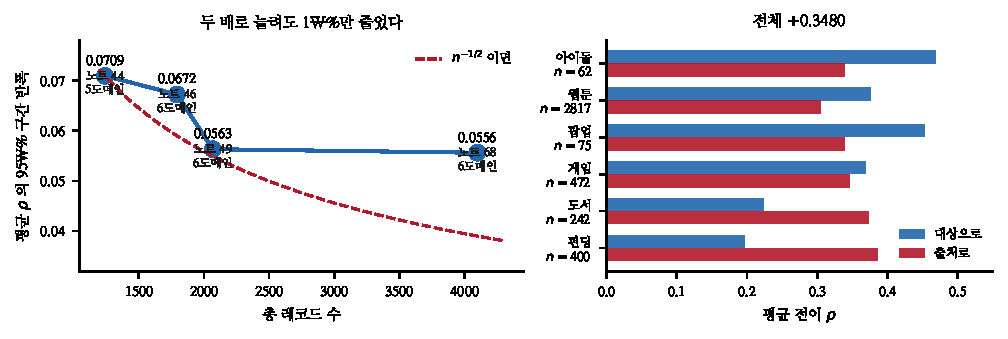
\includegraphics[width=\textwidth]{figs/saturate.pdf}
\caption{왼쪽 --- 표본과 구간 반폭. 오른쪽 --- 현재 도메인별 성적.}
\end{figure}

\begin{table}[t]
\centering\tsize
\caption{구간 반폭의 이력.}
\begin{tabular}{lrrr}
\toprule
& 도메인 & 레코드 & 반폭 \\
\midrule
노트 44 & 5 & 1,241 & 0.0709 \\
노트 46 & 6 & 1,794 & 0.0672 \\
노트 49 & 6 & 2,069 & 0.0563 \\
\textbf{노트 68} & 6 & \textbf{4,098} & \textbf{0.0556} \\
\bottomrule
\end{tabular}
\end{table}

레코드가 두 배인데 반폭이 1\% 줄었다. $n^{-1/2}$이면 0.0563$\times\sqrt{2069/4098}=0.040$이어야
한다.

\claimx{한 도메인의 표본을 늘리는 것으로는 구간이 더 이상 안 좁아진다. 노트 49의
``도메인 내 표본도 좁힌다''는 웹툰 553$\to$900건 구간에서만 맞았고 그 위로는
포화한다.}{웹툰이 이미 다른 도메인의 여섯 배라 한계효용이 사라진 것일 수 있다.
작은 도메인(팝업 75건, 아이돌 62건)을 늘리면 다를 것이다.}

\paragraph{산술이 분명하다}
서른 셀 평균의 요동은 여섯 도메인의 공통 요동에 지배된다. 한 도메인의 표본을
늘리면 그 도메인이 낀 열 셀만 안정되고 나머지 스무 셀은 그대로다. 게다가 웹툰이
이미 가장 큰 도메인이라 그 열 셀도 이미 안정돼 있었다.

\begin{quote}\fontsize{9.5}{11.5}\selectfont
\textbf{자를 좁히려면 새 도메인이거나 작은 도메인이다.} 큰 도메인을 더 키우는
것은 이제 값을 안 한다. 그리고 가장 작은 도메인은 팝업(75건)인데 그것은 내부
자산이라 이 루프에서 못 늘린다.
\end{quote}

\section{보류 항목은 여전히 보류다}

\begin{table}[t]
\centering\tsize
\caption{판정을 기다리던 것들. 반폭 0.056 안에 전부 들어 있다.}
\begin{tabular}{lrl}
\toprule
항목 & 효과 & 출처 \\
\midrule
등급 B 제외 & $+$0.0096 & 노트 63 \\
이중 배선 & $+$0.0080 & 노트 51 \\
웹툰 공통/고유 역전 & $+$0.0045 & 노트 57 \\
\midrule
\multicolumn{2}{l}{현재 구간 반폭} & \textbf{0.0556} \\
\bottomrule
\end{tabular}
\end{table}

셋 다 반폭의 6분의 1 이하다. 노트 45가 계산한 대로 이 급을 판정하려면 반폭이
0.005 아래여야 하고, 그러려면 지금 표본의 백 배가 든다. \textbf{이 항목들은
판정하지 않는 것으로 닫는다} --- 데이터를 더 모아 언젠가 재판정하겠다는 계획은
현실적이지 않다.

\section{현재 상태}

\begin{table}[t]
\centering\tsize
\caption{여섯 도메인 4,098건 · 서른 셀.}
\begin{tabular}{lrrrr}
\toprule
도메인 & n & 자기 $\rho$ & 대상으로 & 출처로 \\
\midrule
아이돌 & 62 & $+$0.472 & $+$0.468 & $+$0.339 \\
\textbf{웹툰} & \textbf{2,817} & $+$0.401 & $+$0.376 & $+$0.305 \\
팝업 & 75 & $+$0.368 & $+$0.453 & $+$0.339 \\
게임 & 472 & $+$0.364 & $+$0.369 & $+$0.346 \\
도서 & 242 & $+$0.202 & $+$0.224 & $+$0.373 \\
펀딩 & 400 & $+$0.190 & $+$0.197 & $+$0.386 \\
\midrule
\multicolumn{2}{l}{평균 $\rho$} & \multicolumn{2}{r}{\textbf{$+$0.3480}} &
$[+0.271, +0.382]$ \\
\multicolumn{2}{l}{자기 $\rho$와의 상관} & & $+$0.945 & $-$0.820 \\
\bottomrule
\end{tabular}
\end{table}

노트 33 · 38 · 40의 두 법칙이 유지된다 --- 자기 상관과 대상 전이가 $+$0.945,
출처 전이가 $-$0.820이다. 웹툰이 자기 상관 $+$0.401로 올라오면서 출처 성적이
$+$0.305로 여섯 중 최저가 됐다. \textbf{상충 법칙이 표본을 늘리는 것만으로
다시 나타난다.}

\section{한계}

\begin{itemize}[leftmargin=1.1em,itemsep=0.15em]
\item 포화를 웹툰 한 도메인에서만 봤다. 작은 도메인을 늘리면 다를 것이다.
\item 웹툰 표본 구성이 크게 바뀌었다(완결 0\%$\to$66\%). 크기와 구성을 분리하지
      않았다.
\item 보류 항목을 ``판정하지 않고 닫는다''고 했는데, 그중 하나가 실제로 이득이면
      그만큼 손해다. 셋을 다 채택했을 때의 상한이 $+$0.022라 크지 않다고 보았다.
\item 붓스트랩 200회다. 반폭 추정 자체가 $\pm$0.005쯤 흔들린다.
\item 전체 $\rho$가 $+$0.3506에서 $+$0.3480으로 조금 내렸다. 웹툰 구성 변화
      때문으로 보이지만 확인하지 않았다.
\end{itemize}

\section{다음}

\begin{enumerate}[leftmargin=1.3em,itemsep=0.15em]
\item 일곱째 도메인 --- 자를 좁히는 유일한 길.
\item 작은 도메인(도서 242건, 펀딩 400건)을 늘려 포화가 크기 때문인지 확인한다.
\item 웹툰 배선을 큰 표본에서 처음부터 다시 고른다(노트 67의 남은 항목).
\item 팝업 표본 --- 여전히 모든 한계의 뿌리이고 이 루프 밖에 있다.
\end{enumerate}

\vspace{0.6em}
\hrule height 0.3pt
\vspace{0.5em}
{\footnotesize
\textbf{참고문헌}\\[0.3em]
Kish, L. (1965). \emph{Survey Sampling}. Wiley.\\[0.15em]
Efron, B., Tibshirani, R. J. (1993). \emph{An Introduction to the Bootstrap}.
Chapman \& Hall.\\[0.15em]
Bouthillier, X. et al. (2021). Accounting for variance in machine learning
benchmarks. \emph{MLSys}, 3, 747--769.\\[0.15em]
Standley, T. et al. (2020). Which tasks should be learned together in multi-task
learning? \emph{ICML}, 9120--9132.\\[0.15em]
Ben-David, S. et al. (2010). A theory of learning from different domains.
\emph{Machine Learning}, 79(1--2), 151--175.
}

\end{document}
